\section{Lösungen zu Kapitel 3}

\begin{Loesung}[zu Aufgabe \ref{Aufg:Logikgatter}]
Es handelt sich um das AND-Gatter (a), um das OR-Gatter (b) und um das NOT-Gatter (c).
\end{Loesung}


\begin{Loesung}[zu Aufgabe \ref{Aufg:OrMasche}]
Sind beide Eingänge auf 0, so sind die Widerstände über den Transistoren sehr groß und die Spannungsabfälle über den Transistoren so groß im Vergleich zum Widerstand unten, dass der Hauptteil der Versorgungsspannung über den Transistoren abfällt. Demnach ist der Ausgang auf logisch 0.

Ist mindestens einer der Eingänge auf 1, so ist der Widerstand des entsprechenden Transistors klein und folglich der Spannungsabfall nur sehr gering. Laut Maschensatz ist auch der Spannungsabfall des anderen Transistors sehr gering. Entsprechend ist vor dem unteren Widerstand noch viel Spannung übrig und der Ausgang liegt auf logisch 1.
\end{Loesung}


\begin{Loesung}[zu Aufgabe \ref{Aufg:NANDNORTransistor}]
\hfill \par \vspace*{-.7cm}
\begin{center}
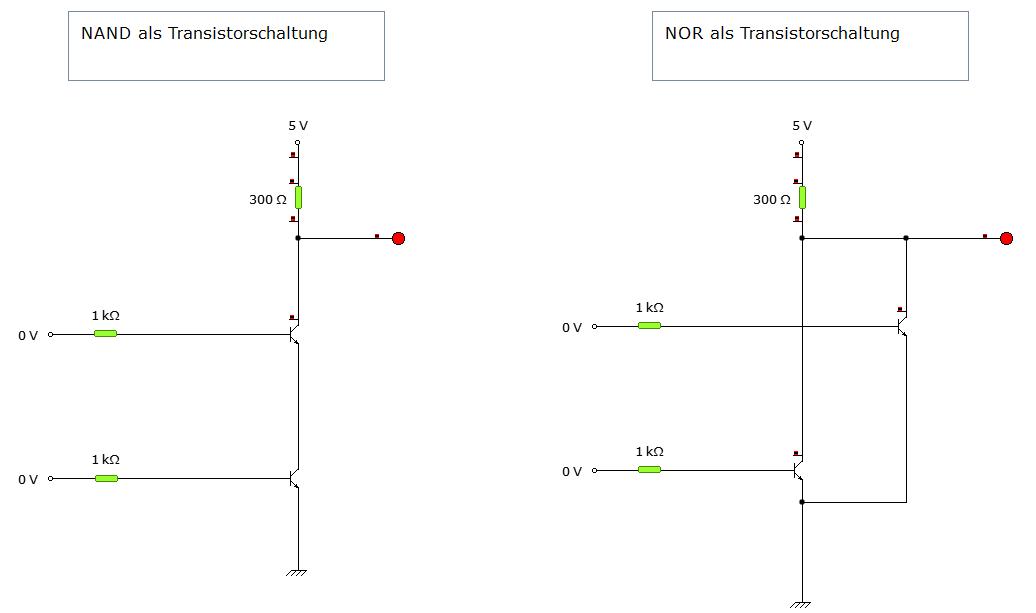
\includegraphics[scale=.6]{pics/Kap3/NANDNOR}
\end{center}
\end{Loesung}


\begin{Loesung}[zu Aufgabe \ref{Aufg:NANDNORTerm}]
\begin{tabular}{cc}
NAND-Gatter: & NOR-Gatter: \\
\begin{tabular}{|c|c||c}
\hline
$a$ & $b$ & $\neg(a \wedge b)$ \\
\hline \hline
0 & 0 & 1 \\
0 & 1 & 1 \\
1 & 0 & 1 \\
1 & 1 & 0 \\
\hline
\end{tabular}
&
\begin{tabular}{|c|c||c}
\hline
$a$ & $b$ & $\neg(a \vee b)$ \\
\hline \hline
0 & 0 & 1 \\
0 & 1 & 0 \\
1 & 0 & 0 \\
1 & 1 & 0 \\
\hline
\end{tabular}
\end{tabular}
\end{Loesung}